\chapter{Testing and Improvements} \label{Testing and Improvements}

\section{Collecting Mechanism}

    While testing the cow dung collecting system we observed that the scraping mechanism was not able to scrape the dung from the tip of the front scraper. So we moved the front roller shaft forward by attaching rods using welding to the existing main frame at the same angle. The original and improved main frame is shown in the figure below.

\begin{figure}[H]
  \centering
    \begin{minipage}{0.40\textwidth}
    \centering
      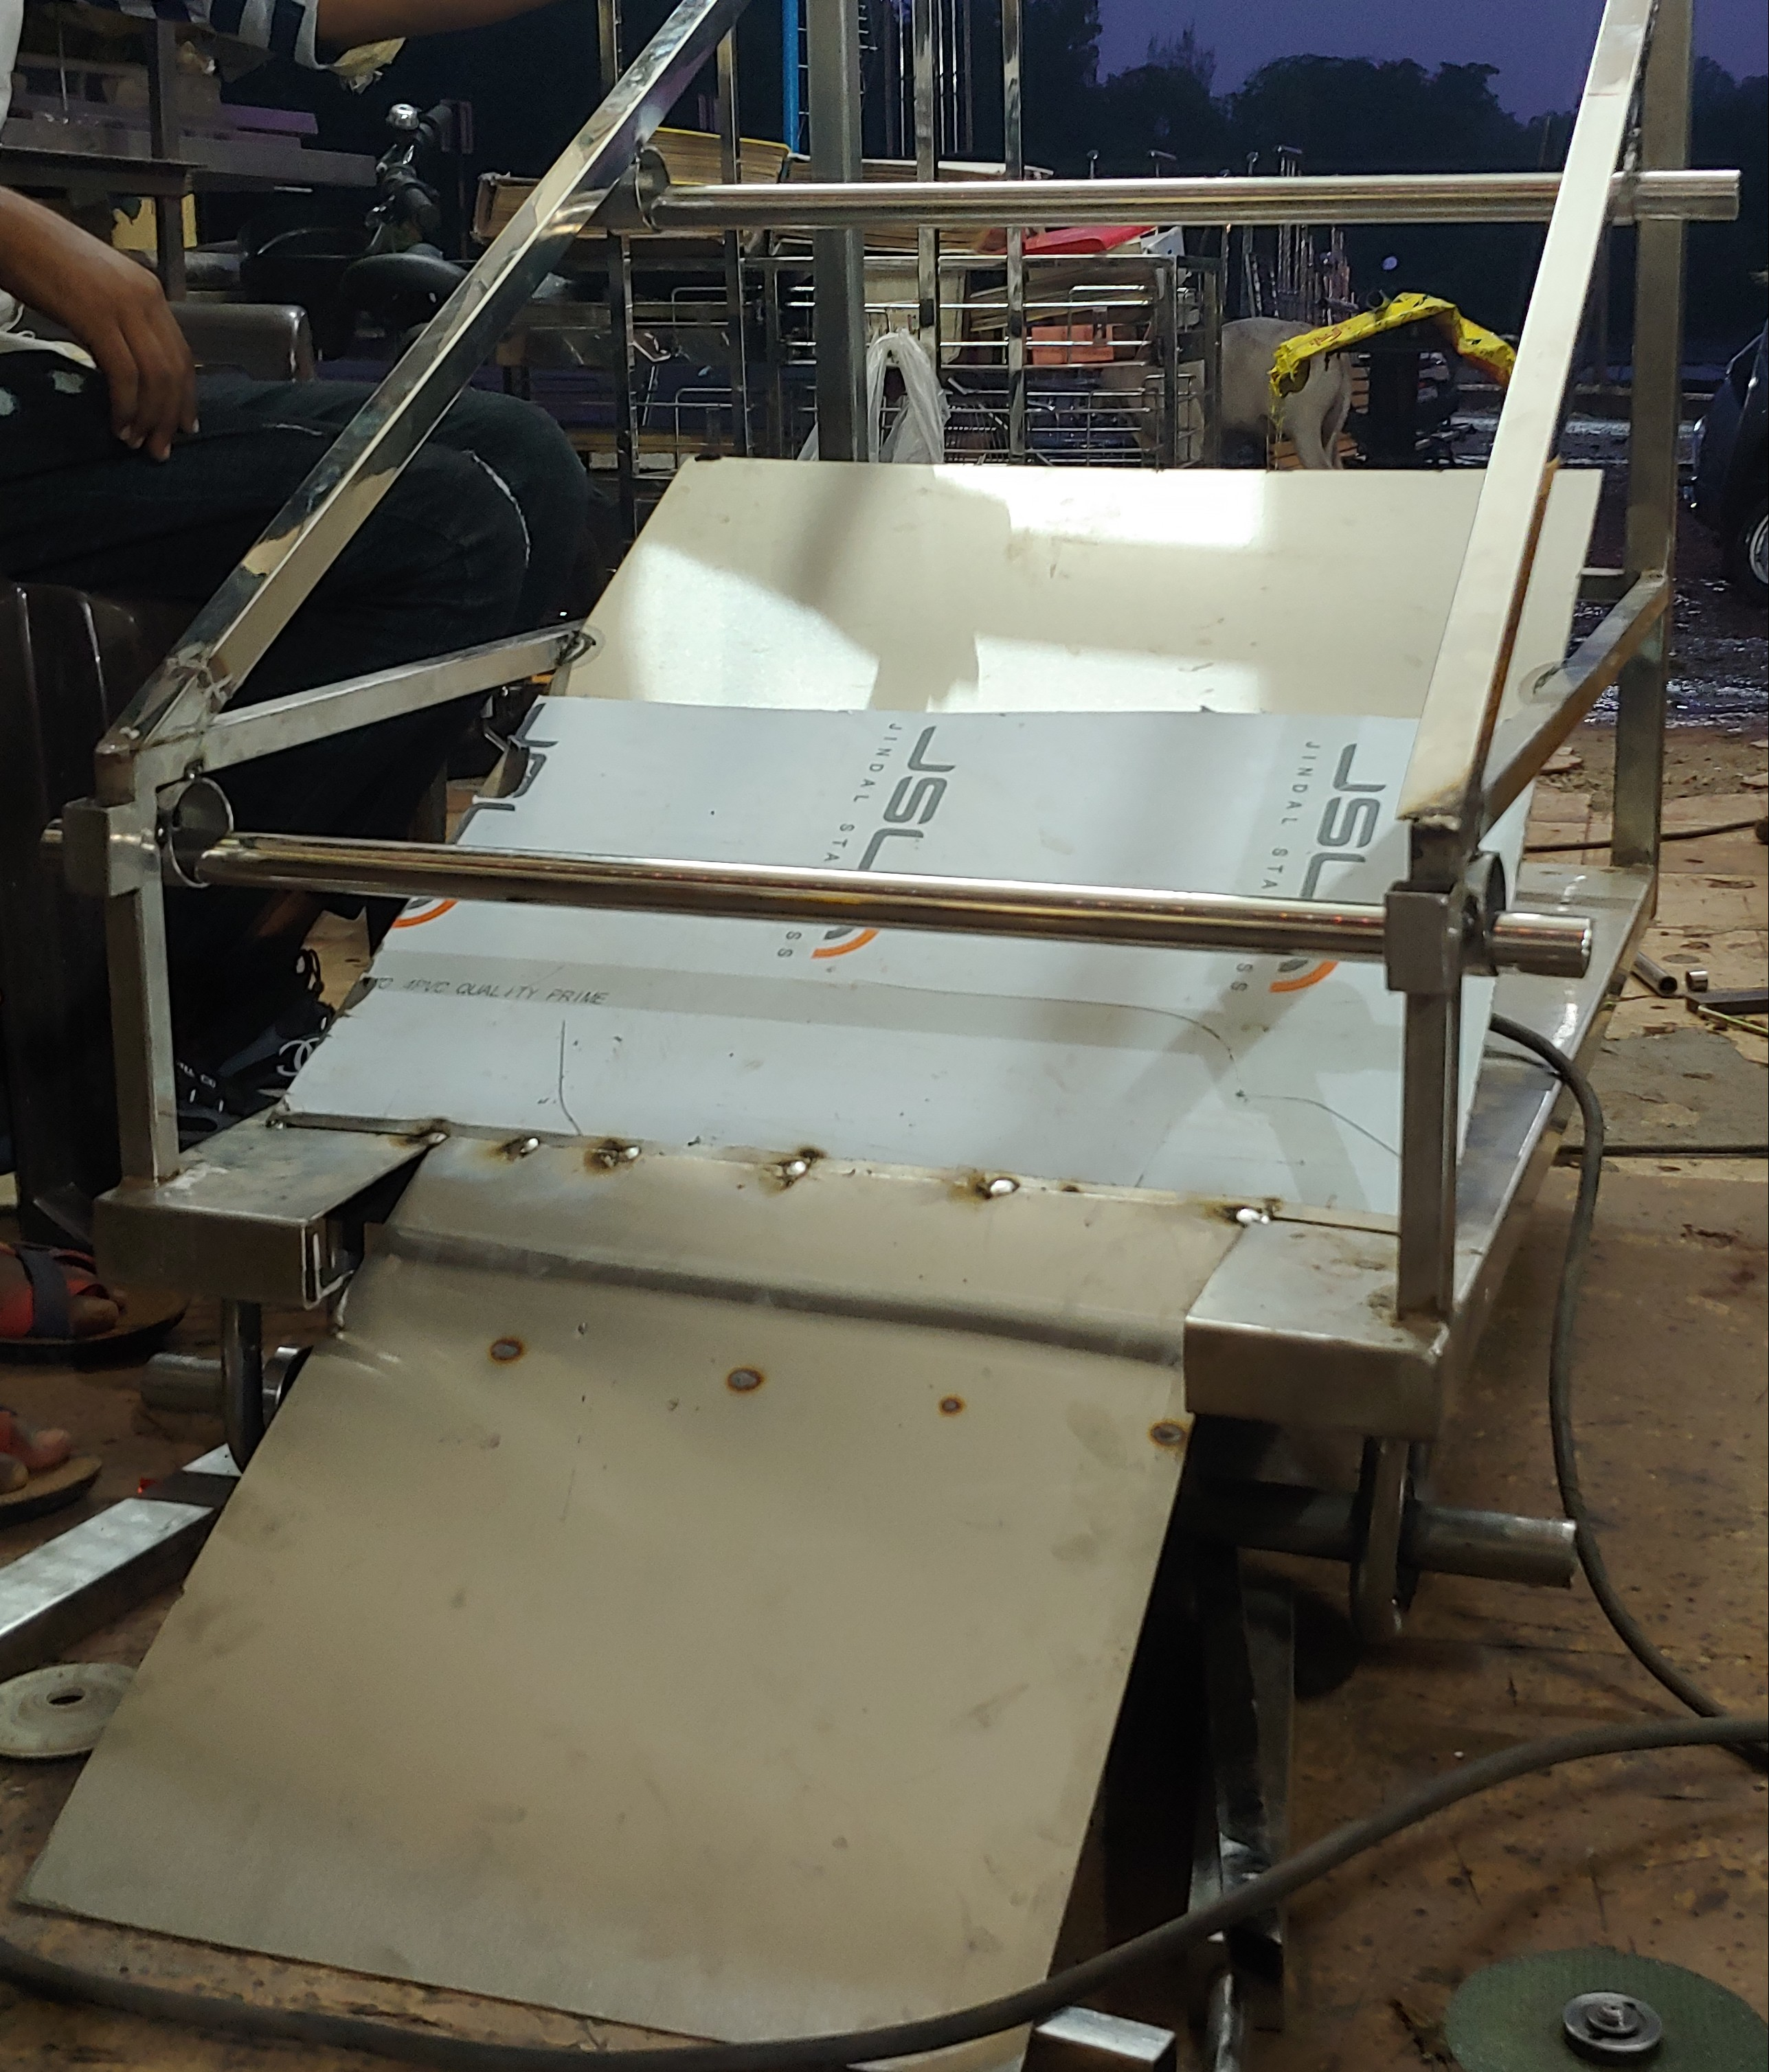
\includegraphics[width=1\textwidth]{Original.jpg}
      \caption{Original}
      \label{fig:Original}
    \end{minipage}
    \begin{minipage}{0.40\textwidth}
    \centering
      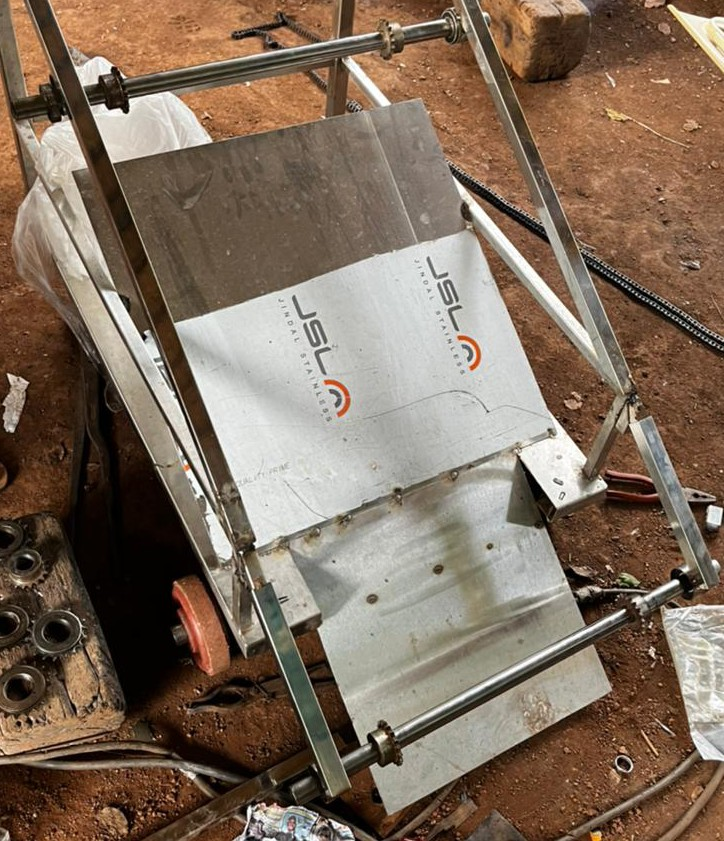
\includegraphics[width=1\textwidth]{Improved.jpg}
      \caption{Improved}
      \label{fig:Improved}
    \end{minipage}
\end{figure}

\section{Bottom Plate}

The bottom plate was designed such that a rectangular hole was provided on it for cow dung to fall inside the bucket once it is scraped by the blades of the scraping mechanism from the front scraper till the hole.

This design was made to achieve additional welding points for the bottom plate for better stability. But during analysis it was observed that same stability could be achieved with less weld points by designing the bottom plate only till the hole which reduced it's weight.

\begin{figure}[H]
  \centering
    \begin{minipage}{0.40\textwidth}
    \centering
      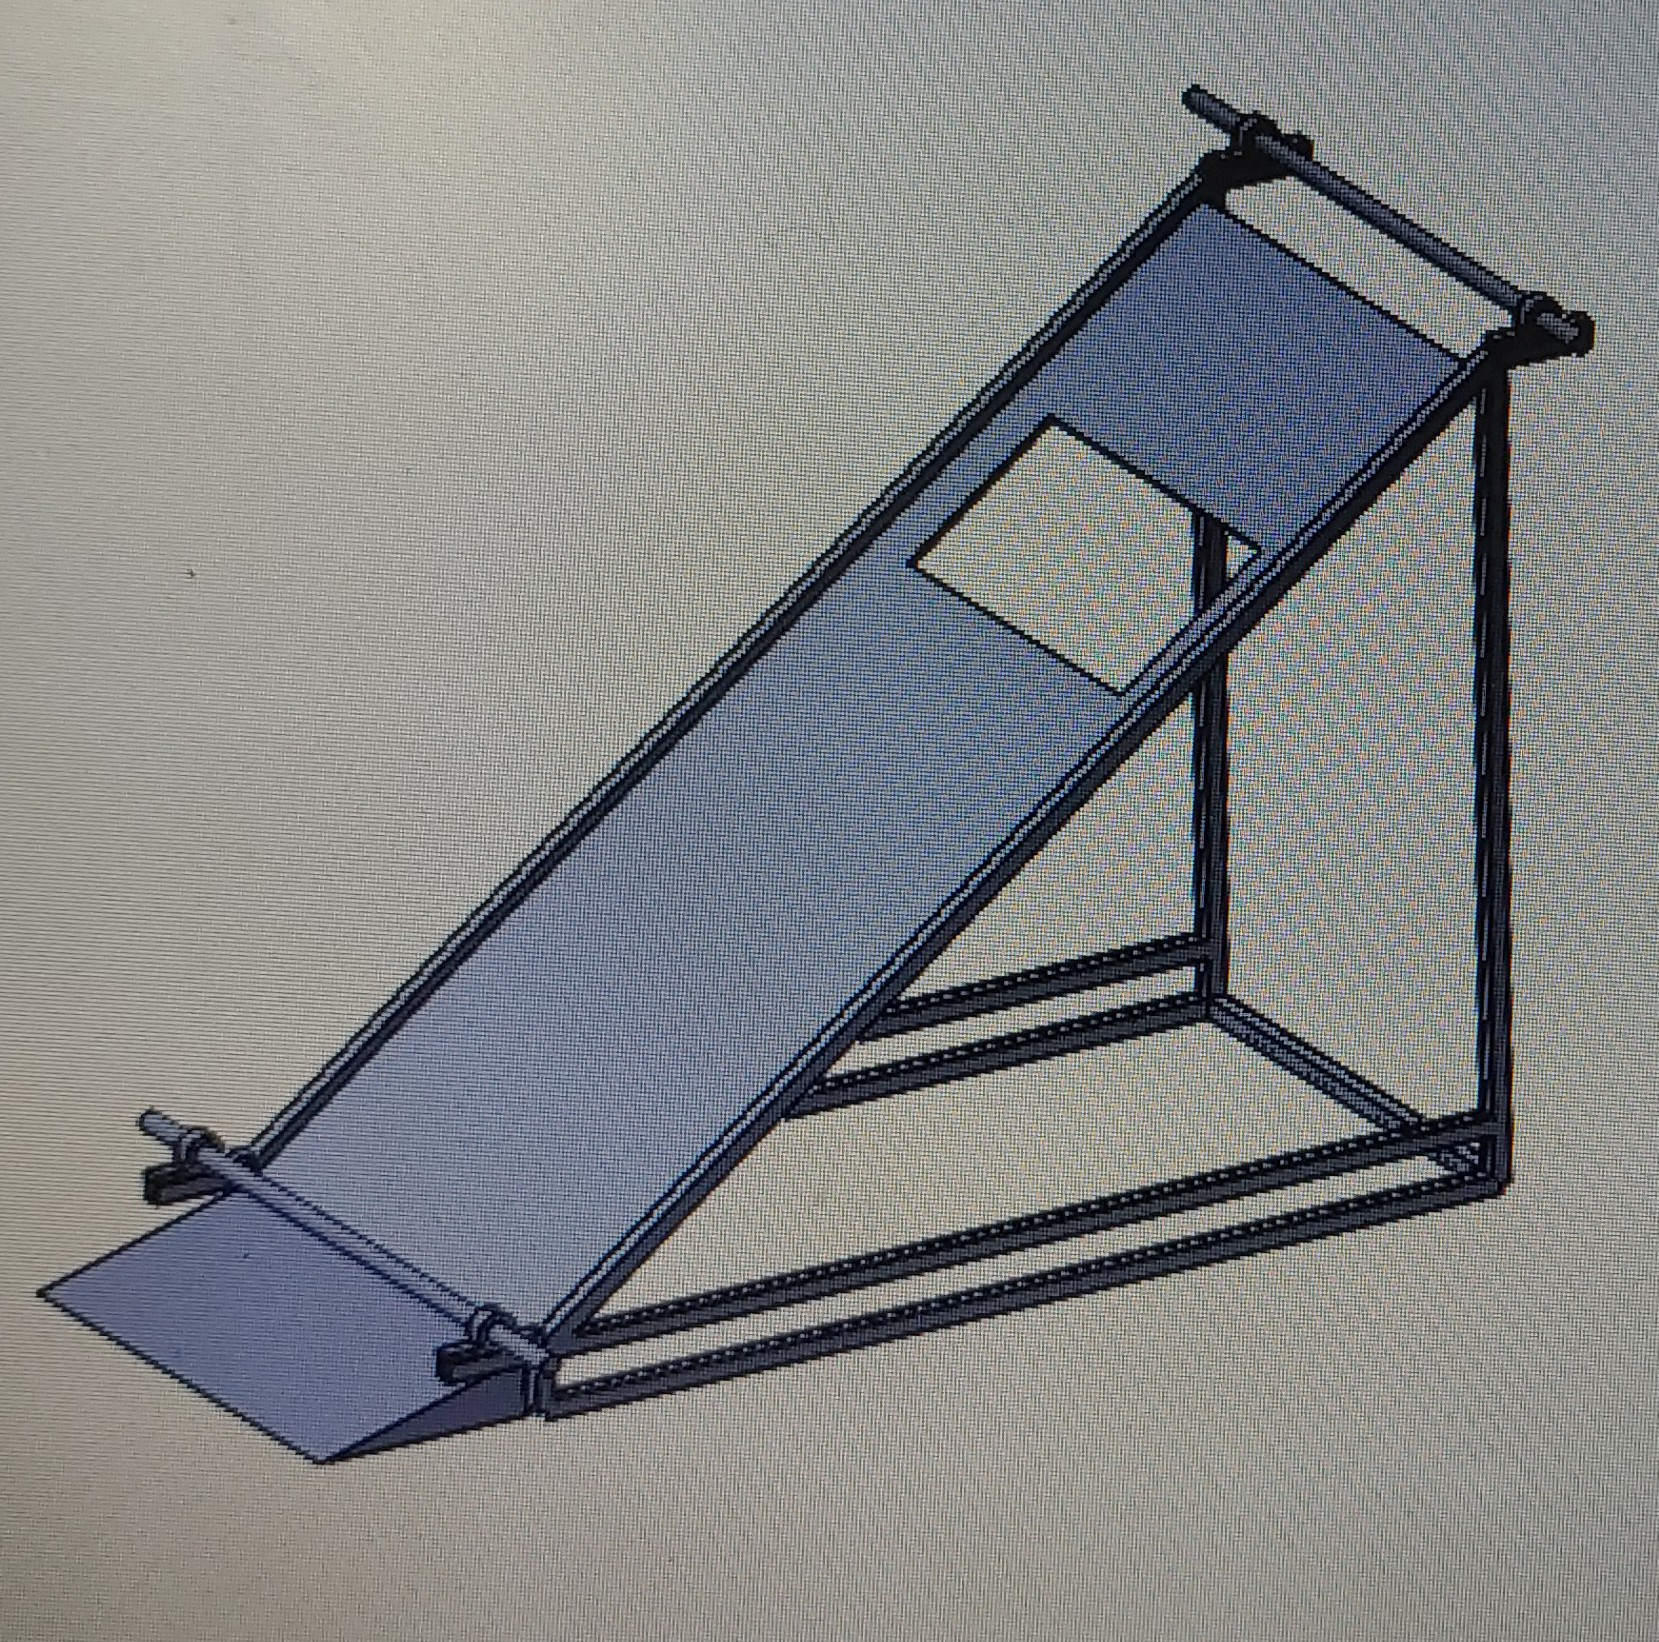
\includegraphics[width=1\textwidth]{Original 1.jpg}
      \caption{Original}
      \label{fig:Original 1}
    \end{minipage}
\hfill
    \begin{minipage}{0.40\textwidth}
    \centering
      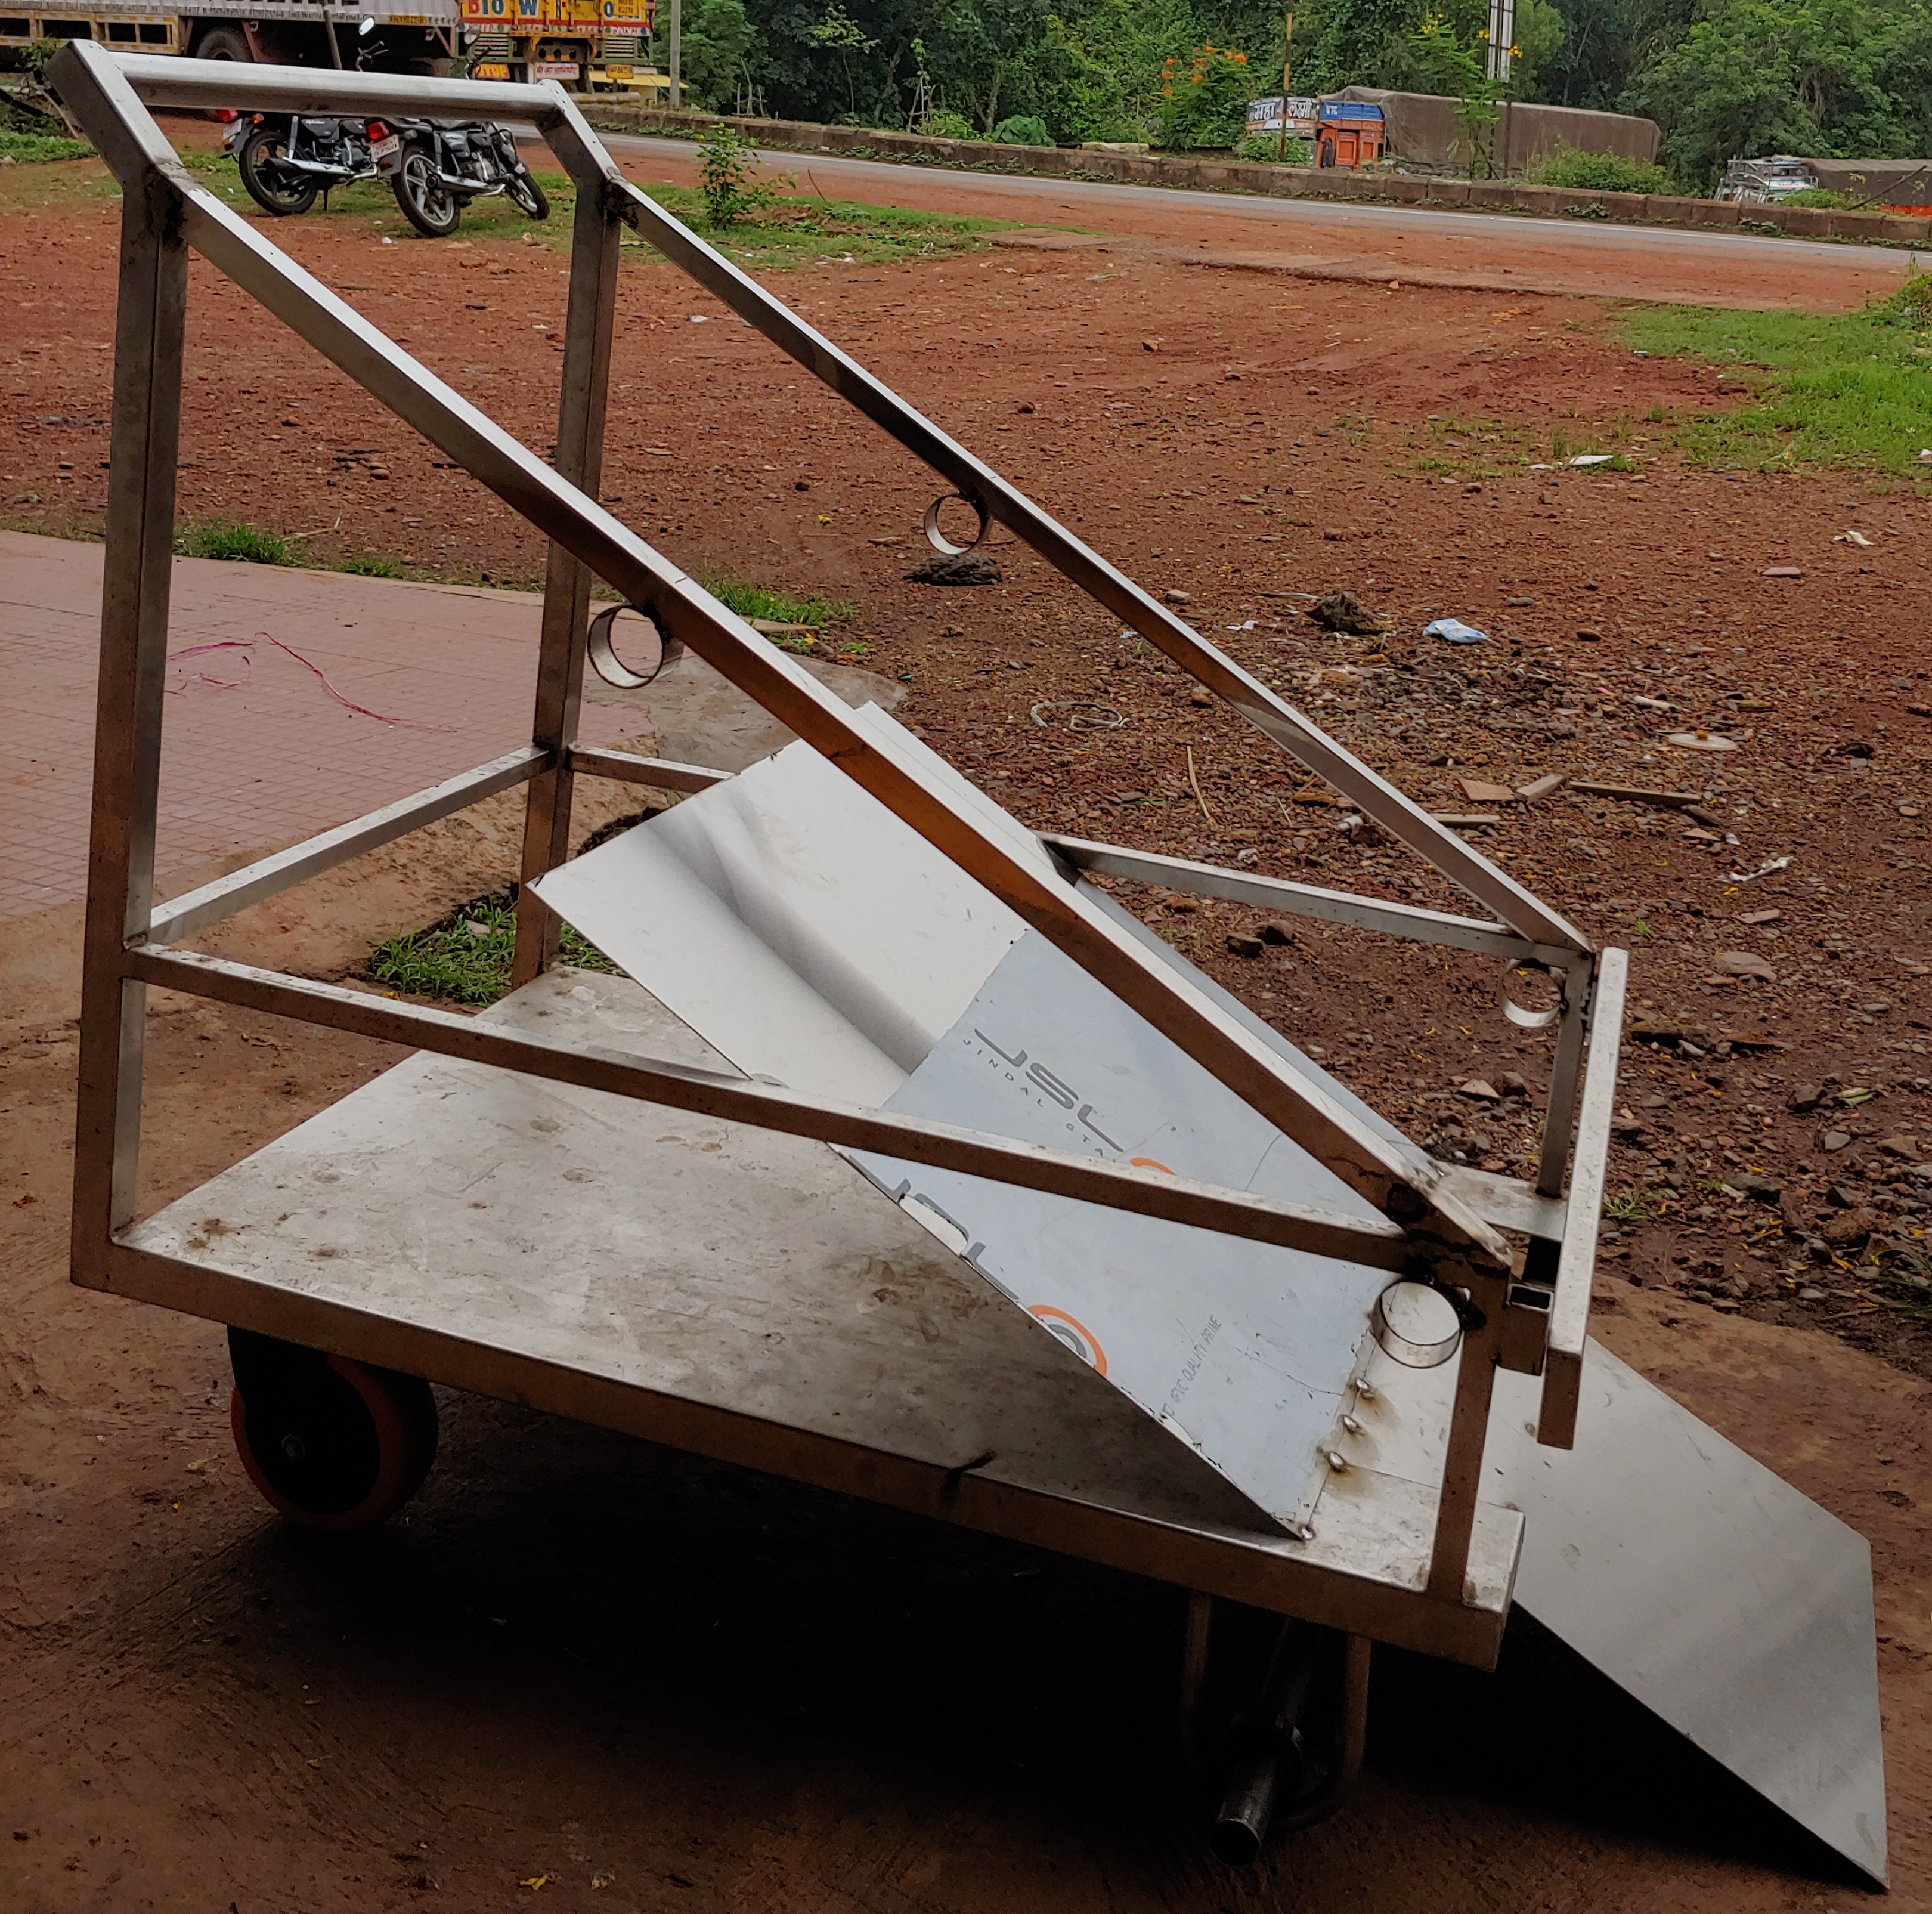
\includegraphics[width=1\textwidth]{Improved 1.jpg}
      \caption{Improved}
      \label{fig:Improved 1}
    \end{minipage}
\end{figure}





\section{Adjustability Mechanism}

    Adjustability mechanism was implemented to quickly and easily adjust the slack of the collecting mechanism chain by finely drifting the front auxiliary shaft. This allowed for quick removal of the shaft too, which made repairing the mechanism quite easier. The mechanism is shown in the figure below.
   
\begin{figure}[H]
  \centering
    \begin{minipage}{0.40\textwidth}
    \centering
      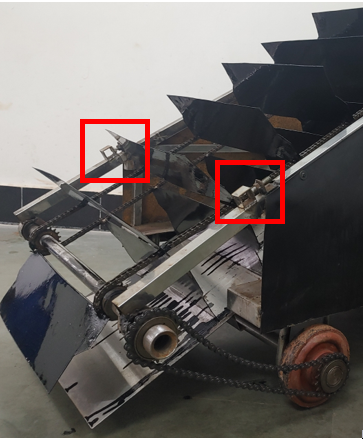
\includegraphics[width=1\textwidth]{adj ass.PNG}
    \end{minipage}
\hfill
    \begin{minipage}{0.50\textwidth}
    \centering
      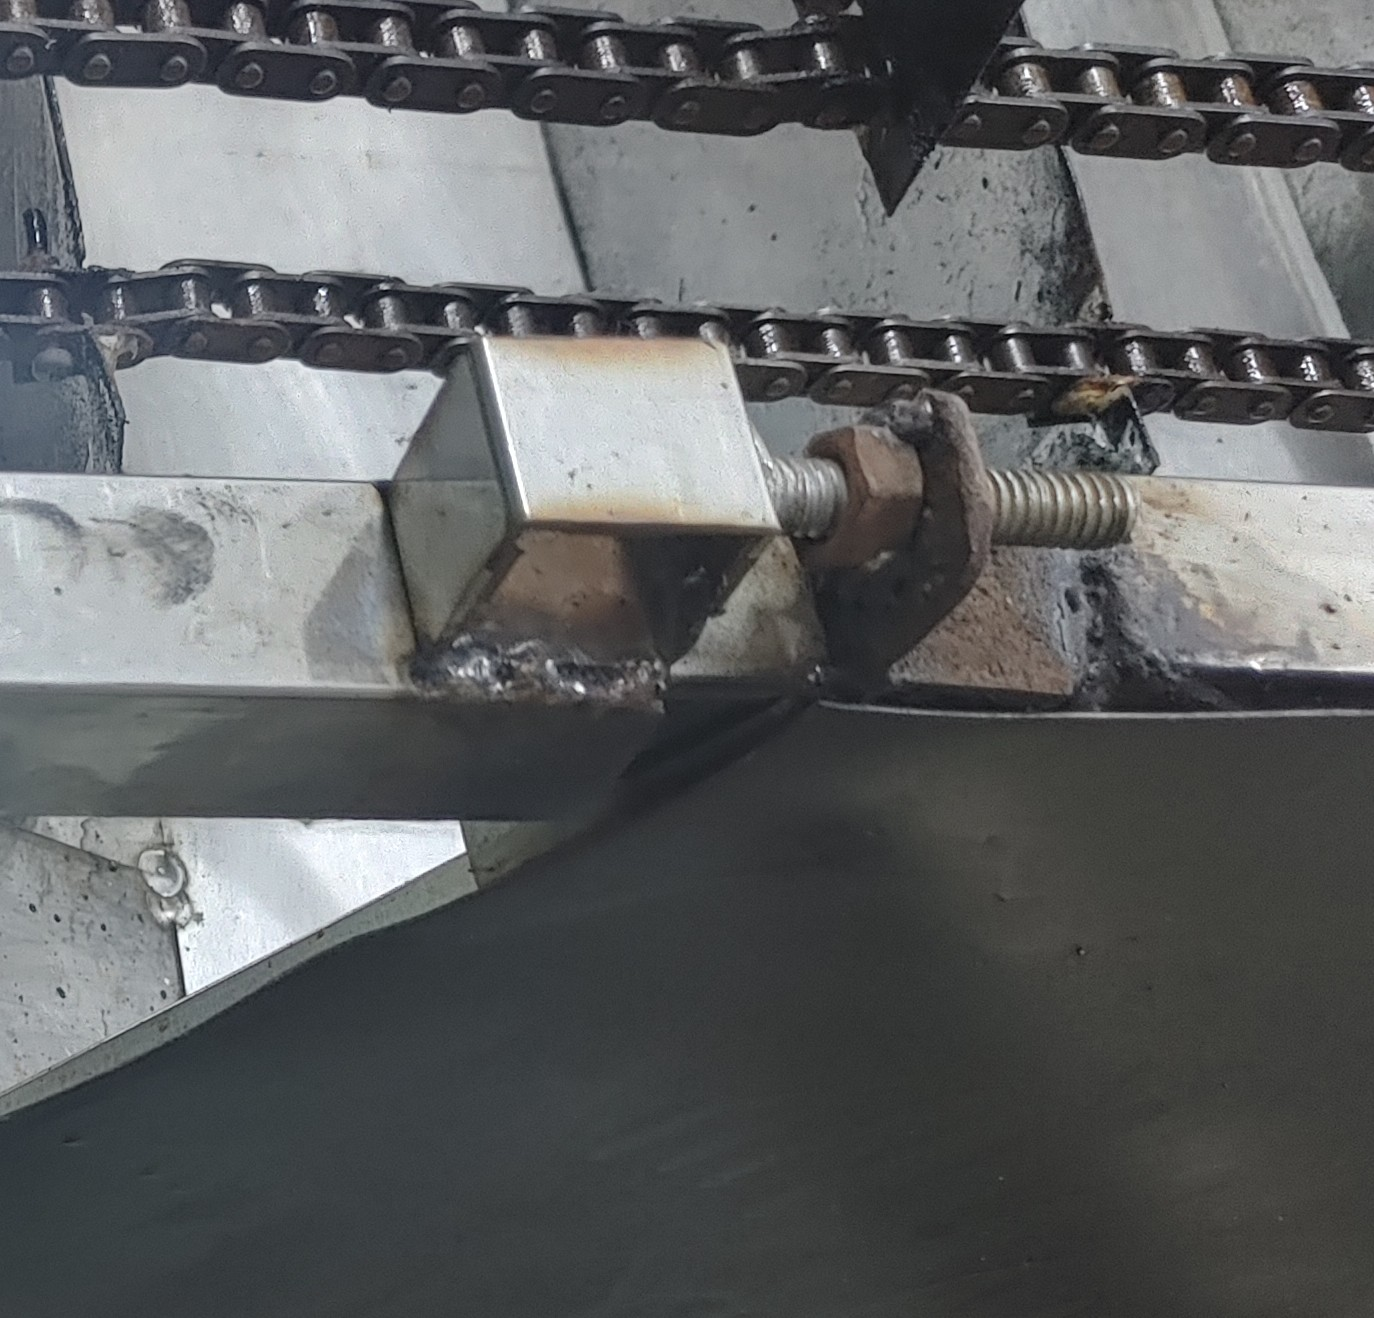
\includegraphics[width=1\textwidth]{Adjustability Mechanism.jpg}
    \end{minipage}
    \caption{Adjustability Mechanism}
\end{figure}
